\chapter{Implementación}

Esta sección estará dedicada a explicar aspectos tanto de la creación y desarrollo de los algoritmos de medición en las pruebas como del resto de elementos de la aplicación, señalando pequeños detalles que hayan podido generar problemas o que tengan alguna relevancia.

\section{Funcionamiento del acelerómetro}
\label{sec:acc}

Antes de proceder con el diseño e implementación de los algoritmos de medición para las pruebas del test SPPB, es importante comprender qué es el acelerómetro, qué mide y cómo funciona.

El acelerómetro es un pequeño sensor que incorporan la gran mayoría de los teléfonos vendidos hoy en día. Su cometido es medir \textbf{cambios en la velocidad de movimiento} del dispositivo que se produzcan en cualquiera de los tres ejes. Es decir, es bueno detectando \textbf{aceleración}.

\begin{figure}[H]
	\centering
	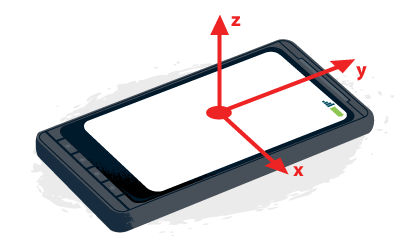
\includegraphics[scale=0.4]{imagenes/axes_mobile.png}
	\caption{Ejes del acelerómetro\label{fig:ejes_acc} \cite{PeteLepage}}
\end{figure}

Si tenemos en cuenta que la gravedad es una fuerza que se mide en unidades de aceleración \cite{gravedad}, podemos obtener también la \textbf{orientación y giros} del dispositivo gracias a la interpretación de la información recibida en cada eje. Por ejemplo si un teléfono móvil está sobre la mesa, recibirá una fuerza en su eje Z similar a la constante de gravedad que genera la tierra, y unos valores cercanos a cero en los ejes X e Y representados en la figura \ref{fig:ejes_acc}.

Por intentar buscar un equivalente, el acelerómetro obtiene datos parecidos a si nosotros tuviésemos los ojos vendados. Al ser movidos, podríamos detectar en qué dirección nos llevan y la orientación de nuestro cuerpo, pero no en qué lugar estamos ni la altitud.

\section{Test de levantarse de la silla}

Este fue probablemente el test más complejo de desarrollar. Como hemos mencionado anteriormente, no es posible detectar la posición ni la altura del dispositivo mediante el uso exclusivo del acelerómetro. Por ejemplo, si el usuario se encuentra de pie o sentado y no se mueve, siempre que el móvil esté sujeto a la zona requerida para este proyecto (el pecho, con orientación vertical) no habrá forma de inferir cual de las dos mencionadas posiciones es la vigente. La razón es que el eje Y marca el mismo valor de gravedad en ambas situaciones mientras que los ejes X y Z marcan cero. La única forma por tanto de determinar la posición actual del usuario sería medir los cambios de aceleración producidos en el proceso de levantarse o sentarse. 

\begin{figure}[H]
	\centering
	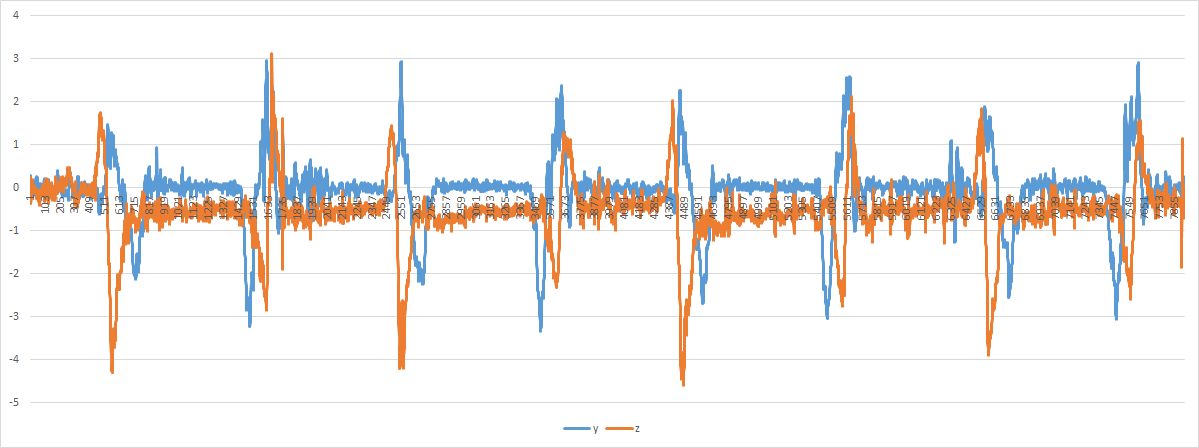
\includegraphics[scale=0.395]{imagenes/grafico_completo_silla_vacio.png}
	\caption{Datos del acelerómetro al levantarse y sentarse.\label{fig:acc_1}}
\end{figure}

Si nos fijamos en la imagen superior (figura \ref{fig:acc_1}) podemos apreciar una gráfica de datos obtenidos por el acelerómetro de un teléfono. La recolección de datos se ha llevado a cabo gracias a una aplicación llamada \textit{``Physics Toolbox Accelerometer''}\cite{Vieyra}. En la gráfica hemos representado solamente los ejes Y (azul) y Z (naranja) por ser los únicos que muestran cambios significativos en el desarrollo del test.

\begin{figure}[H]
	\centering
	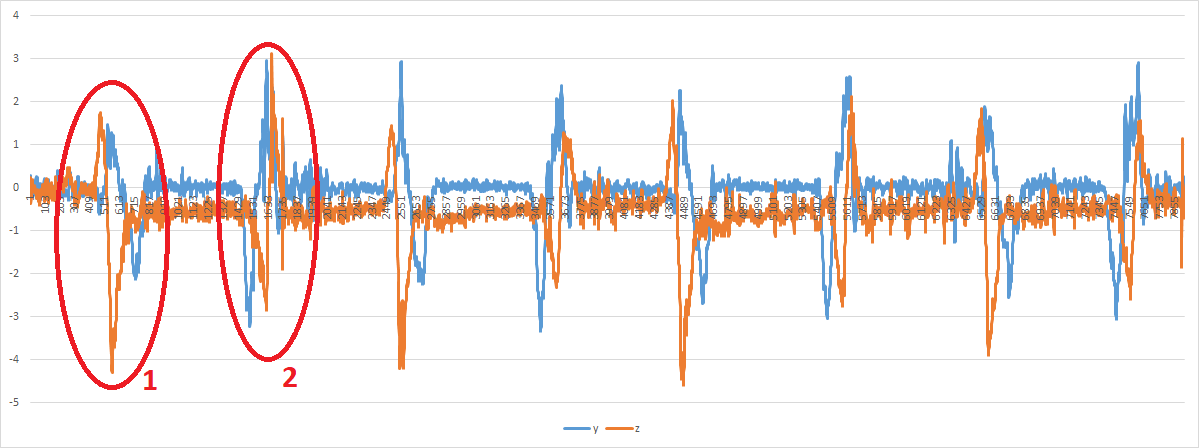
\includegraphics[scale=0.395]{imagenes/grafico_completo_silla.png}
	\caption{Datos del acelerómetro al levantarse y sentarse 2.\label{fig:acc_2}}
\end{figure}

La medición de la gráfica tuvo lugar comenzando desde una posición origen sentado, con lo que los cambios apreciables en la etiqueta 1 corresponden al proceso de levantarse, mientras que los de la etiqueta marcada con un 2 equivalen a sentarse de nuevo. Todas las fluctuaciones intermedias que tienen lugar son debidas en su gran mayoría a ruido en los datos.

Durante el resto de la gráfica, aunque no esté etiquetada, se repite el proceso de levantarse y sentarse hasta en tres ocasiones más. Si lo analizamos más a fondo, podemos encontrar un patrón en los datos de forma relativamente sencilla. Usaremos gráficas con ejes representados individualmente para analizarlos mejor.

\begin{figure}[H]
	\centering
	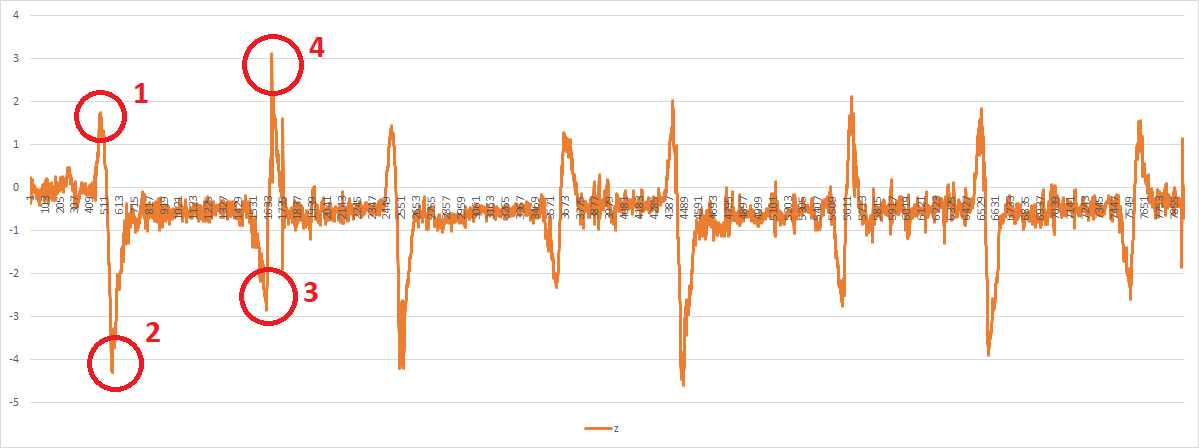
\includegraphics[scale=0.395]{imagenes/grafico_z_silla.png}
	\caption{Datos del acelerómetro al levantarse, eje Z.\label{fig:acc_3}}
\end{figure}

Al levantarnos desde una silla, todo nuestro tronco superior (y con él, el móvil) avanza hacia el frente. Este movimiento de avance, que corresponde al eje Z de nuestro dispositivo mientras lo tengamos sujeto al pecho, se aprecia en la etiqueta 1 de la figura \ref{fig:acc_3}. En ella se llega a alcanzar un pico de casi 2 m/$s^{2}$ de aceleración que al detenerse, provoca una aceleración inversa del dispositivo señalada en la etiqueta número 2.

Cuando procedemos a sentarnos, el tronco se desplaza hacia atrás, provocando un movimiento negativo en el eje Z. Esto encaja con la representación de la etiqueta 3, en la que se ve una aceleración negativa cercana a los -3 m/$s^{2}$, con su correspondiente aceleración inversa al detenerse (una vez sentados completamente) que figura en la etiqueta 4.

Si nos fijamos, los cambios registrados al levantarse y sentarse siguen el mismo patrón pero con signo opuesto. Además, este patrón se repite una y otra vez durante el resto de la gráfica: siempre que hay una aceleración positiva y justo después una negativa, se habrá producido un movimiento de avance en el eje Z necesario para incorporarse, y siempre que haya una aceleración negativa inmediatamente seguida por una positiva, será el movimiento de retroceso (típico al sentarse) el que se haya llevado a cabo.

\begin{figure}[H]
	\centering
	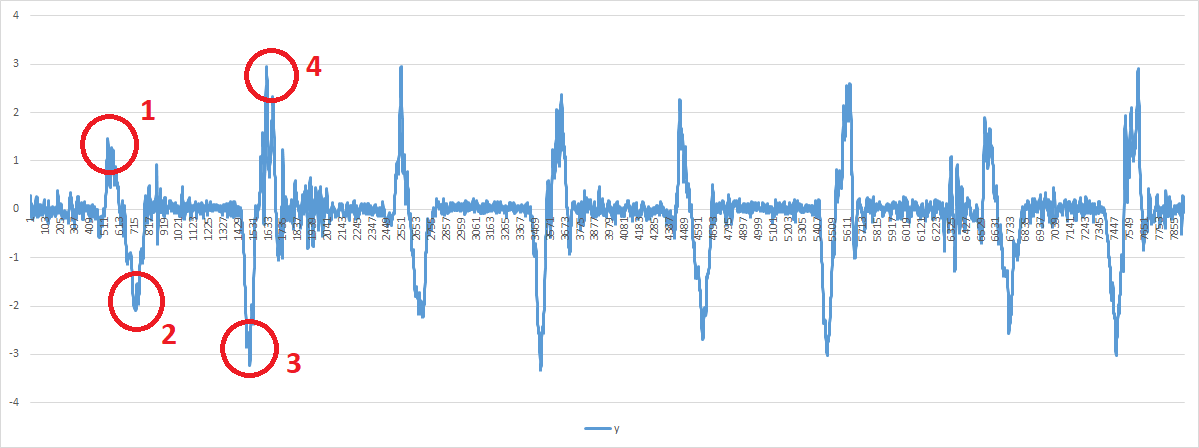
\includegraphics[scale=0.395]{imagenes/grafico_y_silla.png}
	\caption{Datos del acelerómetro al levantarse, eje Y.\label{fig:acc_4}}
\end{figure}

Los datos del eje Y que aparecen en la figura \ref{fig:acc_4} son casi idénticos a los registrados en el eje Z, salvo por un pequeño desfase entre ambos debido principalmente a que solemos inclinarnos hacia delante antes de levantarnos, y empezamos a sentarnos antes de desplazarnos hacia atrás.

Por lo demás, el comportamiento es el mismo. Al levantarnos, nuestro tronco superior sube y el acelerómetro detecta una aceleración positiva (etiqueta 1). Al detener la subida, se vuelve a obtener aceleración inversa como se ve en la etiqueta 2. El procedimiento se vuelve a repetir con valores inversos al sentarnos.

Aunque en esta gráfica parece muy fácil determinar cuándo el usuario se encuentra de pie y cuándo se ha sentado, la tarea se complica bastante en los siguientes casos.

\newpage

\begin{figure}[H]
	\centering
	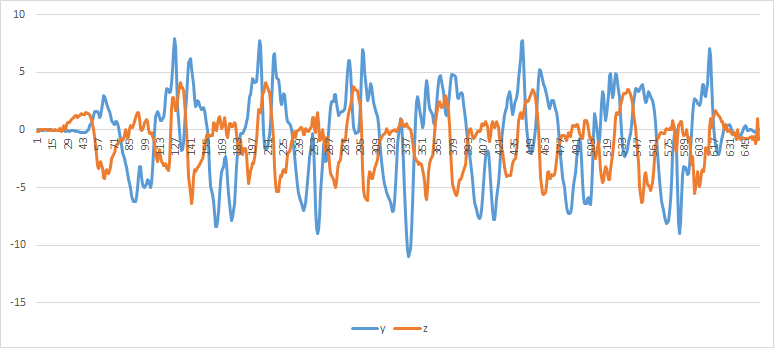
\includegraphics[scale=0.6]{imagenes/grafico_rapido.png}
	\caption{Datos del acelerómetro al realizar movimiento rápidamente.\label{fig:acc_5}}
\end{figure}

Por una parte, si la prueba se desarrolla con demasiada velocidad como se observa en la figura \ref{fig:acc_5}, la aceleración inversa que siempre tiene lugar al finalizar el desplazamiento puede llegar a unirse a la aceleración del  movimiento próximo, provocando un comportamiento más complejo de clasificar, o incluso llegando a presentar fallos.

\begin{figure}[H]
	\centering
	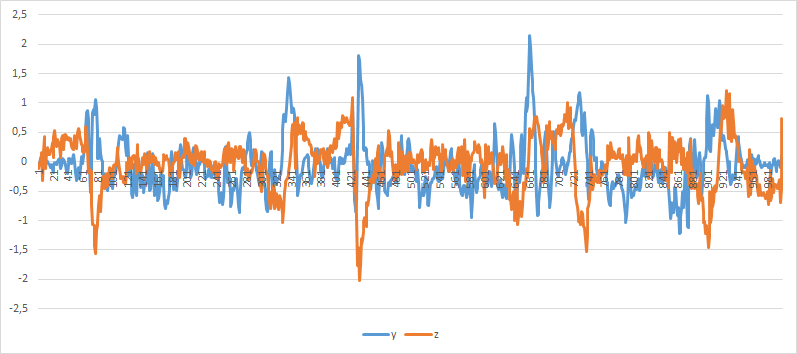
\includegraphics[scale=0.6]{imagenes/grafico_lento.png}
	\caption{Datos del acelerómetro al realizar movimiento lentamente.\label{fig:acc_6}}
\end{figure}

Por otra parte, al efectuar los desplazamientos de forma demasiado pausada (figura \ref{fig:acc_6}), los picos en los datos destacan tan poco que en ocasiones es fácil confundirlos con el propio ruido del acelerómetro, dando también lugar a fallos en algunas ocasiones. A esto hay que añadir que la precisión del sensor puede variar entre distintos dispositivos.

La mejor forma de solucionar estas adversidades sería, a falta de hacer un análisis más profundo, crear un clasificador que determine por sí mismo a qué estado se asemeja más cada patrón de datos. Sin embargo, debido a que la complejidad se escaparía de los objetivos marcados para este proyecto y también a la ausencia de \textit{datasets} suficientemente amplios con datos de acelerómetros atados al pecho durante la ejecución de esta prueba, nos hemos visto obligados a optar por el desarrollo de un algoritmo más convencional y que se desenvuelva de forma aceptable respecto a nuestros requisitos.

El funcionamiento consiste básicamente en pedir al usuario de forma ordenada que se levante y se vuelva a sentar dos veces, de forma que se miden los valores que registra el acelerómetro, se calcula la media y se guardan. Posteriormente, el usuario es libre de levantarse y sentarse hasta alcanzar las cinco repeticiones exigidas por la prueba. 

Para realizarla, se ha de empezar desde la posición sentado tanto por ser un requisito propio del test como por facilitar la medición. Cuando comience a levantarse, si supera las marcas guardadas en los ejes Z e Y durante el calibrado, se determina que se ha levantado una vez. De igual forma se procede para detectar cuándo se ha sentado el usuario.

En la práctica, el algoritmo es ligeramente más complejo ya que tiene en cuenta cuándo se inicia el movimiento y cuándo se detiene. También se reducen las marcas a superar ya que es de esperar que no siempre se acometa con la misma velocidad, a lo que se suma un tiempo de espera pequeño tras cada cambio de posición ayudando a descartar por ejemplo la aceleración producida por un rebote al sentarse bruscamente en la silla. Como el orden siempre ha de ser el mismo (sentado, levantado, sentado, etc.), no es necesario calcular completamente en qué postura se encuentra el usuario en todo momento, sino más bien determinar si ha pasado a la siguiente posición o no. No obstante eso no es suficiente para evitar errores de medición en la totalidad de casos.

Debido a la dificultad de solventar estos problemas completamente, se decidió añadir la opción de realizar la prueba con el dispositivo en el muslo. La gran diferencia es que cuando nos sentamos, el eje Y se encuentra en posición horizontal y al levantarnos, en vertical, lo cual facilita mucho la medición y reduce enormemente la posibilidad de obtener fallos independientemente de la velocidad a la que se realice u otros factores. Puede apreciarse mejor en la siguiente figura (\ref{fig:acc_muslo}), donde se representa la fuerza de la gravedad sobre el eje Y:

Cuando estamos sentados, la gráfica muestra una fuerza de gravedad cercana a cero en el eje Y, lo cual tiene sentido respecto a la organización de los ejes de coordenadas en la imagen \ref{fig:ejes_acc} del apartado \ref{sec:acc}.

En cambio, al estar de pie toda la fuerza de la gravedad recae sobre dicho eje, haciendo que su valor alcance unas cotas cercanas a uno mientras se mantenga en esa posición. Que los números sean positivos o negativos indica únicamente si el teléfono se encuentra con la parte superior hacia arriba o hacia abajo, lo cual es irrelevante para la prueba y puede ser descartado trabajando con el valor absoluto.

\begin{figure}[H]
	\centering
	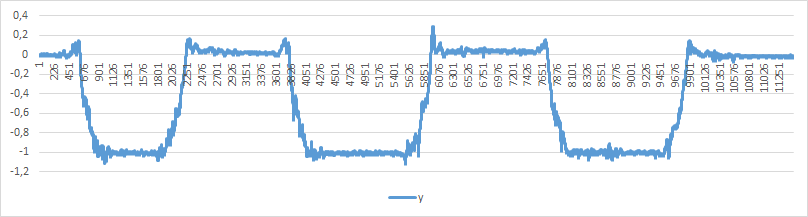
\includegraphics[scale=0.6]{imagenes/grafico_y_muslo.png}
	\caption{Datos del acelerómetro en el muslo.\label{fig:acc_muslo}}
\end{figure}

\section{Test de equilibrio}

El algoritmo desarrollado para la medición de este test es relativamente simple. Se sustenta en el hecho de que mientras se está manteniendo el equilibrio, los datos obtenidos por los tres ejes del acelerómetro deberían permanecer más o menos constantes. 

Lo que se hace es pedir al usuario que se sitúe en la posición origen (de pie, con los pies juntos) con el dispositivo en el pecho y se mantenga inmóvil hasta finalizar el calibrado. Dicho calibrado consiste básicamente en guardar los datos de todos los eje de coordenadas que devuelve el acelerómetro y hacer la media de cada uno de ellos durante unos cuantos segundos. En la gráfica de la siguiente imagen (figura \ref{fig:acc_7}) se ha mantenido el equilibrio hasta aproximadamente la mitad de la prueba, donde se aprecia de forma clara un despunte por encima de lo habitual en cualquiera de los ejes. Esto demuestra que en principio es fácil determinar el fin del test.

\begin{figure}[H]
	\centering
	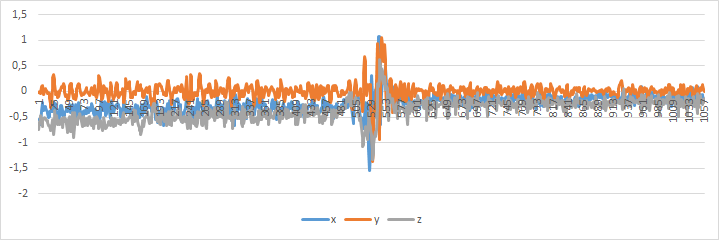
\includegraphics[scale=0.65]{imagenes/grafico_equilibrio.png}
	\caption{Datos del acelerómetro al romper equilibrio.\label{fig:acc_7}}
\end{figure}

Una vez iniciado el test, si la medición en alguno de los tres ejes excede significativamente la media calculada durante su calibración, se establece que el usuario se ha movido, se calcula la puntuación en base al tiempo transcurrido y se finaliza la prueba.

\begin{lstlisting}[language=Java]
if (calibrated && inProgress) {
    // How much the current value changes with respect to the average or
    // normal position.
    float change_x, change_y, change_z;
    change_x = Math.abs(x - mean_x);
    change_y = Math.abs(y - mean_y);
    change_z = Math.abs(z - mean_z);

    long elapsedMillis = SystemClock.elapsedRealtime() - chronometer.getBase();

    if(change_x > move_allowed || change_z > move_allowed || change_y > 1) {
        desbalanced(elapsedMillis);

    } else if (elapsedMillis > 10100) {
        chronometer.stop();
        iv_person.setImageResource(R.drawable.ic_test_done);
        continueTest();
    }
}
\end{lstlisting}

Como vemos en la línea 14 del código superior, al superar los 10.000 milisegundos (10 segundos), se finaliza la prueba y se llama a los métodos correspondientes para indicárselo al usuario y continuar con el test.

\section{Test de velocidad de marcha}

En este test nos hemos centrado en crear un algoritmo que determine el tiempo que el usuario se está moviendo. Hemos descartado para ello llevar la cuenta de los pasos dados o cualquier otro dato que dificultase la medición.

La única información utilizada ha sido la proporcionada por el eje Y. En la siguiente figura (número \ref{fig:acc_8}) vemos un patrón sencillo en el que cada despunte del gráfico equivale a un paso del usuario. Para obtener estos datos se estaba utilizando también el giroscopio, un sensor que no muchos móviles de gama baja incorporan, con lo que se optó por prescindir de él y reemplazar la información utilizando exclusivamente el acelerómetro. Aunque en la gráfica parece muy fácil determinar los pasos, la tarea se puede volver más compleja si el usuario tiene una movilidad limitada y camina muy lento o de forma muy suave.

\begin{figure}[H]
	\centering
	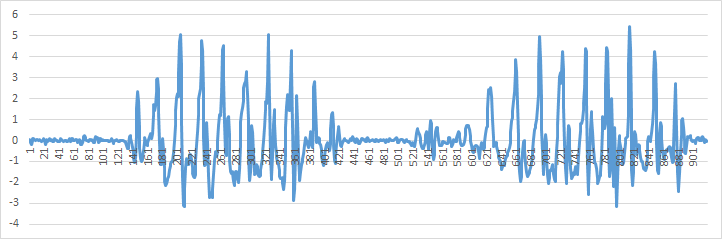
\includegraphics[scale=0.65]{imagenes/grafico_andar.png}
	\caption{Datos del acelerómetro al andar.\label{fig:acc_8}}
\end{figure}

El funcionamiento del algoritmo es el siguiente. Una vez iniciada la prueba, se empieza a contar el tiempo transcurrido y se almacena el máximo valor del eje Y obtenido hasta el momento. Con cada paso, este valor puede actualizarse si supera el máximo anterior. En caso de no superarse, si la aceleración en el eje Y es al menos mayor que un tercio del máximo registrado, se determina que el usuario está aún caminando. Cuando no se supere este valor durante un tiempo determinado (dos segundos en este caso), se señala el fin de la prueba y se calcula el tiempo total que el usuario ha estado caminando.

\begin{lstlisting}[language=Java]
if (yChange > max_change/3f){
    lastChangeTime = curTime;
    if(yChange > max_change) {
        max_change = yChange;
    }
}
\end{lstlisting}

\section{Lista de usuarios}

La lista de usuarios que aparece en la sección \textit{Usuarios} (figura \ref{fig:capturas_usuarios}) se creó en un primer momento utilizando un componente de Android denominado \textbf{ListView}. Lo que hace ListView es leer una serie de elementos (que en este caso son los usuarios guardados en la base de datos local) y mostrarlos en una lista desplazable, utilizando para ello un \textit{adaptador}. Sin embargo, se trata de un elemento algo antiguo y el funcionamiento era lento y presentaba tirones a pesar del pequeño número de usuarios que estaba mostrando. 

Por ello, se decidió sustituir ListView por el más reciente \textbf{RecyclerView}, otro componente con un objetivo prácticamente idéntico pero con un funcionamiento subyacente diferente. Mientras que ListView genera una vista nueva para cada uno de los elementos mostrados, Recyclerview reutiliza las vistas creadas para otros elementos no visibles, lo que resulta en un menor gasto de recursos y un funcionamiento más suave.

Se añadió también la posibilidad de eliminar cualquiera de los usuarios almacenados mediante un gesto llamado \textit{Swipe} o Deslizar, gesto que pudo conseguirse implementando la clase RecyclerUserTouchHelper. Al arrastrar el usuario a eliminar, se descubre un fondo rojo con un icono de papelera y un texto que indica la acción a acometer. Normalmente este fondo se crea en el momento de arrastrar ya que así se pueden añadir funciones diferentes en función de la dirección en la que se realice, sin embargo optamos por la idea de diseñar el fondo directamente en el archivo de interfaz de los objetos de lista ya que presentaba menos errores que la otra opción.

Por último, se han implementado acciones para responder tanto a un click largo sobre alguno de los usuarios almacenados, que lo señala y guarda como seleccionado (o deseleccionado si ya lo estaba), y un click o toque corto, que abre el fragmento de puntuación y lo actualiza con toda la información rescatada de la base de datos respecto al ID de usuario clicado. Estas acciones en conjunto ofrecen un comportamiento mucho más dinámico de la lista además de añadir utilidad real que mejora y amplía la experiencia de usuario.

Para guardar un usuario, al presionar el botón dedicado a tal fin y rellenar el cuadro de diálogo que aparece, se ejecutan las siguientes acciones que permiten insertar los datos obtenidos en la base de datos. Como podemos ver en la línea 3, se crea un objeto usuario a través de su constructor siendo necesario únicamente insertar el nombre que tendrá, el cual ha sido comprobado anteriormente para evitar guardar una cadena vacía. Una vez creado el objeto, se introduce en la base de datos a través del método \textit{insert} de la línea 4, que será desglosado también a continuación. También se hace en este paso la acción de marcar como seleccionado el usuario recién creado entre las líneas 6 y 8. Por último, se actualiza el componente Recyclerview para que muestre el nuevo objeto.


\begin{lstlisting}
String userName = edt.getText().toString();
if (userName.length() != 0) {
    User user = new User(edt.getText().toString());
    user.insert(getActivity());

    selectedId = user.getId();
    editor.putLong(SELECTED_USER, selectedId);
    editor.apply();

    showUsersList();
}
\end{lstlisting}

El método \textit{insert} de la clase \textit{User} que hemos comentado anteriormente lleva a cabo las siguientes acciones. En primer lugar guarda las variables del objeto en cada uno de los campos correspondientes para su almacenado (líneas 3-8). Posteriormente, crea un objeto de la clase \textit{LocalSQLiteOpenHelper} para acceder a la base de datos, obtiene ``permisos'' de escritura e inserta los valores anteriores en la tabla correspondiente. En último lugar (línea 14) nos aseguramos de cerrar el acceso a la base de datos.

\begin{lstlisting}
public void insert(Context context) {
    ContentValues values = new ContentValues();
    values.put(UsersDB.UserEntry.NAME,this.name);
    values.put(UsersDB.UserEntry.BALANCE_SCORE, this.balanceScore);
    values.put(UsersDB.UserEntry.SPEED_SCORE, this.speedScore);
    values.put(UsersDB.UserEntry.CHAIR_SCORE, this.chairScore);
    values.put(UsersDB.UserEntry.TEST_DATE, this.testDate);
    values.put(UsersDB.UserEntry.AVERAGE_SPEED, this.averageSpeed);

    LocalSQLiteOpenHelper helper = new
            LocalSQLiteOpenHelper(context);
    SQLiteDatabase db = helper.getWritableDatabase();
    this.id=db.insert("USERS", null, values);
    db.close();
}
\end{lstlisting}

El funcionamiento de los métodos utilizados para actualizar la información de algún usuario o para eliminarlo es similar al que acabamos de ver, con lo que no los comentaremos. 

\section{Pantalla de puntuación}

En la figura \ref{fig:capturas_puntuacion} vemos la pantalla de puntuación. Queríamos crear un entorno para mostrar los resultados del usuario que fuese bonito y dinámico, pero a la misma vez limpio y fácil de entender. Para ello, optamos por añadir como primer elemento un círculo que se rellenase con colores en función de la puntuación total alcanzada, a parte de mostrarla en su interior para evitar dudas. 

Este círculo se realizó usando un componente de Android denominado \textbf{ProgressBar}, muy habitual en las pantallas de carga para representar la progresión de las mismas. En nuestro caso el uso era distinto pero se adaptaba igual de bien. Utilizamos elementos XML para cambiar la apariencia y el color de la progresión. También añadimos una animación tanto al progreso de la barra como al del texto para que simulase ser un contador analógico mediante el uso de las clases ValueAnimator y ObjetAnimator.

\begin{lstlisting}
ValueAnimator animator = new ValueAnimator();
animator.setObjectValues(0, score);
animator.addUpdateListener(new ValueAnimator.AnimatorUpdateListener() {
    public void onAnimationUpdate(ValueAnimator animation) {
        tv_score.setText(String.valueOf(animation.getAnimatedValue()));
    }
});
animator.setDuration(2000); 
animator.start();

ObjectAnimator animation = ObjectAnimator.ofInt(progressBar, "progress", pb_score);
animation.setDuration(2000);
animation.setInterpolator(new DecelerateInterpolator());
animation.start();
\end{lstlisting}

Los siguientes elementos de la pantalla de puntuación son estáticos, aunque también se muestran u ocultan en función de las pruebas realizadas por el usuario. Se trata del desglose de la puntuación entre las tres pruebas, cuyo diseño ya analizamos en el capítulo correspondiente.

También aparece aquí un botón que permite salvar la información de los resultados en un usuario determinado, según haya sido seleccionado de forma previa, en caso de que la pantalla de puntuación se muestre tras finalizar un test y no al acceder desde la lista de Usuarios. Para guardar dicha información, se accede a el objeto de la clase Usuario (mUser) seleccionado y se establece la puntuación de cada una de las pruebas realizadas. En último lugar, se hace una llamada a su método \textit{update} el cual se encarga del proceso necesario para insertar la información en la base de datos.

\begin{lstlisting}
if (tv_balance_score.getVisibility() == View.VISIBLE)
    mUser.setBalanceScore(mBalanceScore);
if (tv_gait_score.getVisibility() == View.VISIBLE){
    mUser.setSpeedScore(mGaitScore);
    mUser.setAverageSpeed(mAverageSpeed);
}
if (tv_chair_score.getVisibility() == View.VISIBLE)
    mUser.setChairScore(mChairScore);
mUser.update(getActivity());
\end{lstlisting}

\section{Internacionalización y accesibilidad}

\subsection{Internacionalización}

Todos los recursos de texto que se muestran en la aplicación se encuentran agrupados en un único archivo denominado \textbf{strings.xml}, que abarca tanto títulos como descripciones e instrucciones de voz. Esto permite modificarlos de forma sencilla y rápida, a parte de poder crear archivos paralelos para ser traducidos con el objetivo de que la aplicación se adapte al idioma del mayor número de personas posible.

En la actualidad cuenta con soporte para los idiomas inglés y español de forma automática. Es decir, el lenguaje establecido por defecto en cada dispositivo afectará al lenguaje en el que se muestre la aplicación. Para añadir nuevos idiomas bastará con generar una copia traducida del archivo Strings más reciente. Se ha evitado la inclusión de texto en cualquier imagen para agilizar el proceso de internacionalización, evitando la edición pormenorizada de cada una. 

Además se ha tenido en cuenta a los idiomas con escritura de derecha a izquierda (o RTL por sus siglas en inglés), de forma que el texto adapte correctamente los márgenes y espacios en función a la dirección del mismo. Con la vista puesta en un posible lanzamiento futuro de la aplicación en mercados con esas características, se ahorrará la necesidad de editar el diseño de las múltiples interfaces a posteriori.

\subsection{Accesibilidad}

La aplicación adapta la mayoría de los textos a las preferencias de tamaño establecidas por el usuario. Esto es realmente útil y muy importante en especial para la población anciana, que suele establecer el máximo tamaño de fuente debido a problemas de visión. Además, se ha estudiado el comportamiento de todas las secciones para asegurar que el cambio de tamaño no impide la correcta visualización de los elementos, añadiendo la posibilidad de realizar deslizamientos en aquellas pantallas donde el texto pueda exceder los límites de la misma. 

Por otra parte, también se ha tenido en cuenta el funcionamiento de herramientas de accesibilidad como Talkback, así que todas las imágenes y botones sin texto que requieren de una explicación en caso de no poder ser visualizados tienen su correspondiente descripción en todos los idiomas en los que la app está disponible.

\section{Miscelánea}

Aquí listaremos otras características importantes para el correcto funcionamiento de la aplicación pero que no se muestran a simple vista en la mayoría de casos.

\subsection{Carencia de acelerómetro}

El funcionamiento de todo este proyecto está orientado a la realización del test mediante el sensor acelerómetro de los teléfonos. En caso de que algún dispositivo no cuente con él, pueden presentarse fallos y cierres inesperados si no se trata de forma correcta. 

Por este motivo se decidió mostrar un mensaje al abrir la aplicación en esos casos en los que el móvil no posea el sensor necesario, indicando al usuario la razón por la que la aplicación no puede ser usada. Puede verse en la figura siguiente (\ref{fig:no_acc}).

\begin{figure}[H]
	\centering
	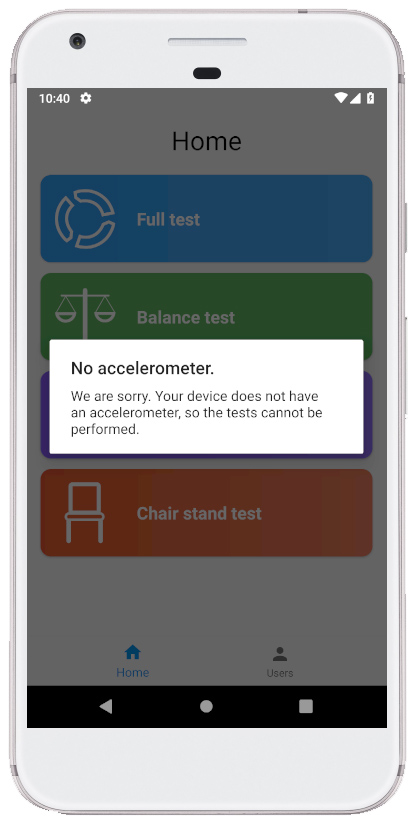
\includegraphics[scale=0.35]{imagenes/no_acc.jpg}
	\caption{No hay acelerómetro.\label{fig:no_acc}}
\end{figure}

\subsection{Posición fija de pantalla}

Debido a que durante la realización del test SPPB el móvil deberá permanecer sujeto al pecho y en una posición concreta (vertical), no tiene sentido que al girar el teléfono la pantalla también gire, provocando además una visualización incorrecta de la interfaz y problemas en la medición. Por esta razón, se ha determinado que todas los fragmentos que aparecen dentro de la actividad TestActivity (\ref{fig:navegacion}) estén fijos en posición vertical, independientemente de la orientación del teléfono. El resto de actividades y fragmentos sí que pueden girar y adaptarse.

\subsection{Evitar bloqueo durante test}
La mayoría de usuarios establece un tiempo tras el cual la pantalla se apaga y el dispositivo se bloquea. Aunque es una buena forma de ahorrar batería, pero que esto suceda durante la ejecución de las pruebas puede dar como resultado la incompletitud de las mismas o todo tipo de fallos.

Para subsanar este problema, se añadió la característica de que la pantalla nunca se apague mientras se encuentre dentro de la actividad TestActivity (\ref{fig:navegacion}), lo que implica que el móvil siempre está activo durante la realización de cualquiera de los tests. Al abandonar dicha actividad, se desactiva esta herramienta y la pantalla recupera su comportamiento habitual.

